\documentclass[letterpaper, 10pt, openany]{memoir}

\usepackage{graphicx}
\usepackage{wrapfig}
\graphicspath{{./images/}}

\setstocksize{6.5in}{5.5in}
\settrimmedsize{6.5in}{5.5in}{*}
\setlrmarginsandblock{1in}{1in}{*}
\setulmarginsandblock{1in}{1in}{*}
\checkandfixthelayout

\setlength\parindent{0pt}

% Title
\pretitle{\begin{center}}

\title{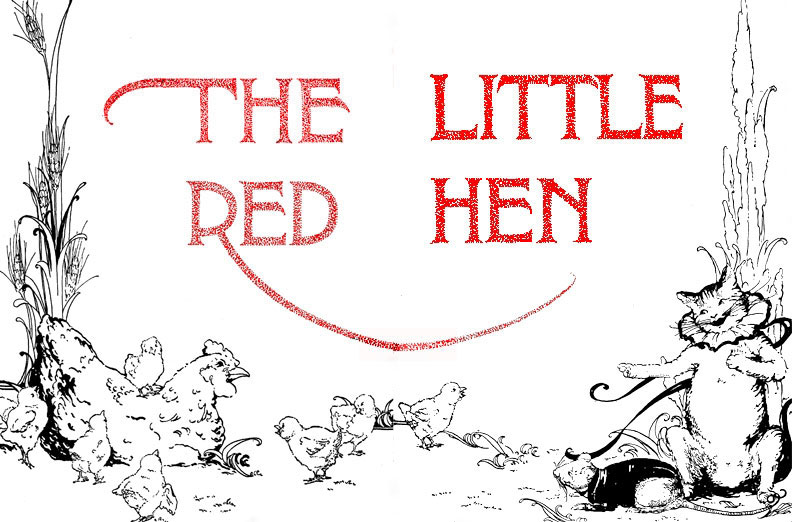
\includegraphics[width=\textwidth]{image_044.jpg}
\newpage
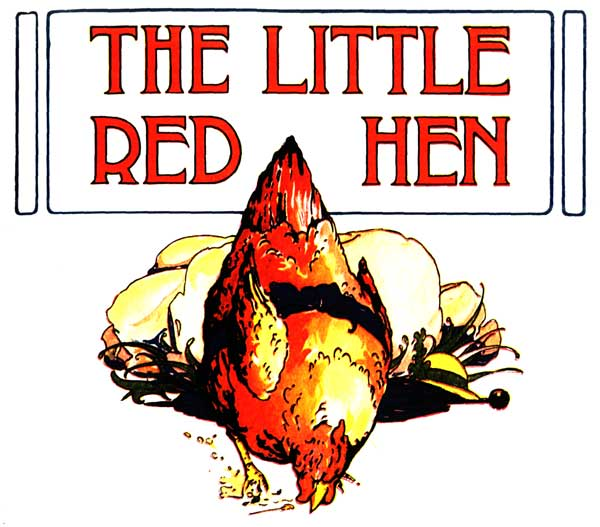
\includegraphics[width=\textwidth]{image_045_1.jpg}
\newpage

\huge{\MakeUppercase{\textbf{The Little Red Hen}}}

\vspace{\onelineskip}

\normalsize{An Old English Folk Tale

\vspace{\onelineskip}
\vspace{\onelineskip}

Retold and Illustrated
\vspace{\onelineskip}

\textbf{by}}}

\posttitle{\end{center}}
\author{\MakeUppercase{\textbf{Florence White Williams}}}
\date{}

\begin{document}

\maketitle

\newpage
\begin{center}
The

\textsc{Saalfield Publishing Company}

\textsc{Chicago - Akron, Ohio - New York}

\vspace{\onelineskip}

\tiny{\MakeUppercase{Printed in U.S.A.}}

\vspace{\onelineskip}

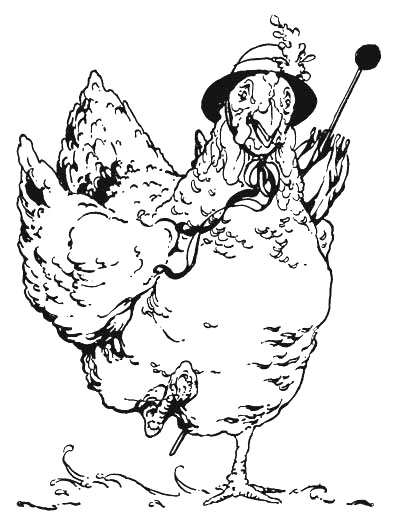
\includegraphics[width=0.7\textwidth]{image_004.jpg}

\vspace{\onelineskip}

COPYRIGHT, 1918

BY

THE SAALFIELD PUBLISHING COMPANY
\end{center}

\newpage
\begin{wrapfigure}[3]{l}{0.15\textwidth}
	
\includegraphics[width=0.15\textwidth]{image_005_1.jpg}
\end{wrapfigure}

Little Red Hen l/ved in a barnyard. She spent almost all of her time walking about the 
barnyard 

\vspace{\onelineskip}

\begin{wrapfigure}[6]{l}{0.6\textwidth}
	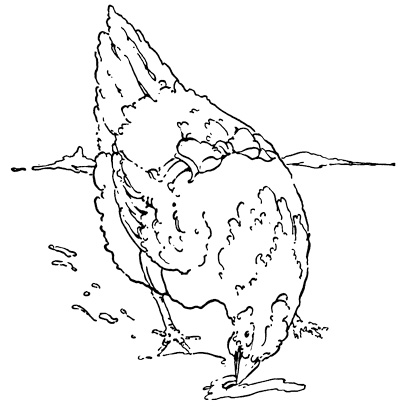
\includegraphics[width=0.6\textwidth]{image_005_2.jpg}
\end{wrapfigure}

in her

\vspace{\onelineskip}

picketty-pecketty

\vspace{\onelineskip}

fashion,

\vspace{\onelineskip}

scratching

\vspace{\onelineskip}

everywhere

\vspace{\onelineskip}

for worms.

\newpage
\begin{wrapfigure}[3]{l}{0.1\textwidth}
	
\includegraphics[width=0.1\textwidth]{image_012_1.jpg}
\end{wrapfigure}

he dearly loved fat, delicious worms and felt they were absolutely necessary to the
health of her children. As often as

\begin{wrapfigure}[6]{r}{0.6\textwidth}
	\vspace{-2\onelineskip}
	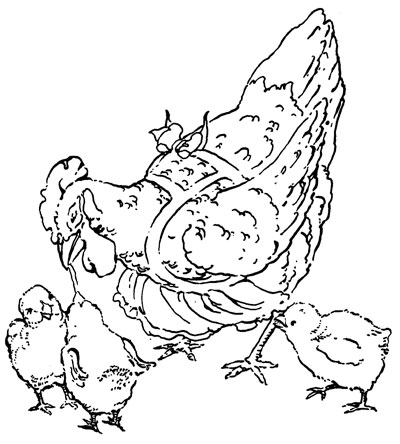
\includegraphics[width=0.6\textwidth]{image_006.jpg}
\end{wrapfigure}

\vspace{\onelineskip}

she

\vspace{\onelineskip}

found a

\vspace{\onelineskip}

worm

\vspace{\onelineskip}

she

\vspace{\onelineskip}

would

\vspace{\onelineskip}

call

\vspace{3\onelineskip}

``Chuck-chuck-chuck!'' to her chickies.

\newpage
\begin{wrapfigure}[3]{l}{0.15\textwidth}
	
\includegraphics[width=0.15\textwidth]{image_007_1.jpg}
\end{wrapfigure}

hen they were gathered about her, she would distribute choice morsels of her tid-bit.
A busy little body was she!

\begin{center}
	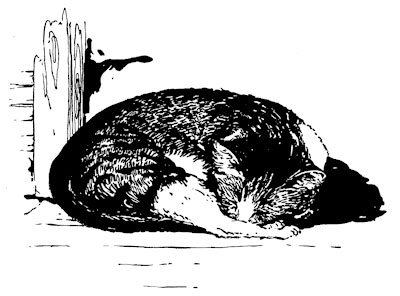
\includegraphics[scale=0.5]{image_007_2.jpg}
\end{center}

\vspace{\onelineskip}

A cat usually napped lazily in the barn door, not even bothering herself to scare the rat
who ran here and there as

\newpage
\begin{wrapfigure}[11]{l}{0.55\textwidth}
	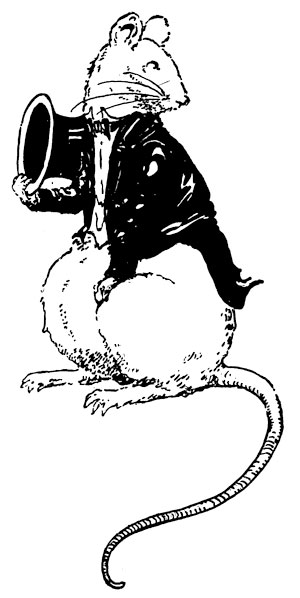
\includegraphics[width=0.55\textwidth]{image_008.jpg}
\end{wrapfigure}
he pleased.

\vspace{\onelineskip}

And

\vspace{\onelineskip}

as for

\vspace{\onelineskip}

the pig

\vspace{\onelineskip}

who lived

\vspace{\onelineskip}

in the

\vspace{\onelineskip}

sty—he

\vspace{\onelineskip}

did

\vspace{\onelineskip}

not care what

\vspace{\onelineskip}

happened so long as he could eat and grow fat.

\newpage
\begin{wrapfigure}[5]{l}{0.15\textwidth}
	
\includegraphics[width=0.15\textwidth]{image_009_1.jpg}
\end{wrapfigure}

ne day the Little Red Hen found a Seed. It was a Wheat Seed, but the Little Red
Hen was so accustomed to bugs and worms that she supposed this to be some new and
perhaps very delicious kind of meat. She bit it gently and found that it resembled
a worm in no way whatsoever as to taste although because it was long and slender, a
Little Red Hen might easily be fooled by its appearance.

\vspace{\onelineskip}

\begin{center}
	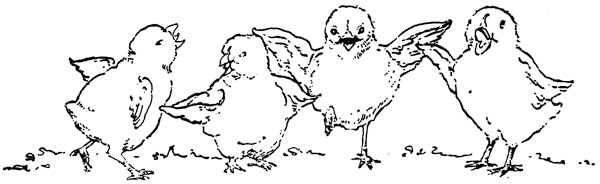
\includegraphics[width=\textwidth]{image_009_2.jpg}
\end{center}

\newpage
\begin{center}
	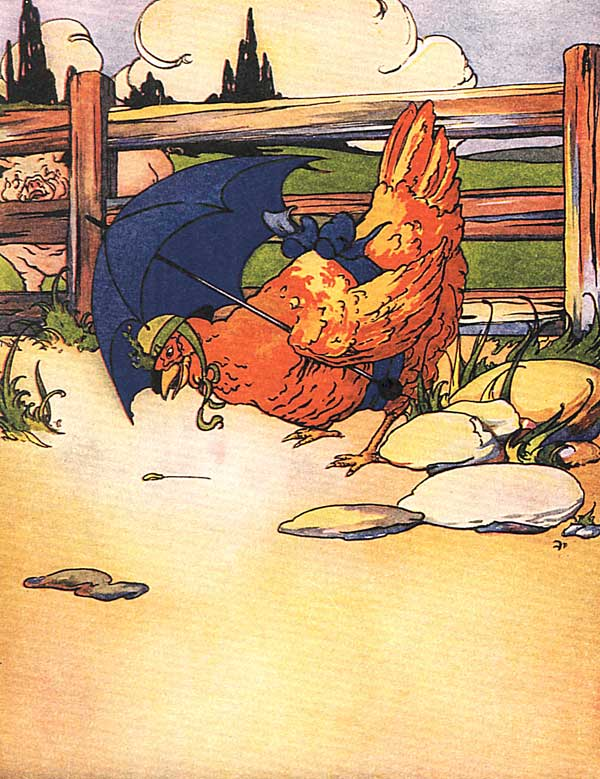
\includegraphics[width=\textwidth]{image_046_1.jpg}
\end{center}

\newpage
\begin{wrapfigure}[5]{l}{0.15\textwidth}
	
\includegraphics[width=0.15\textwidth]{image_011_1.jpg}
\end{wrapfigure}

arrying it about, she made many inquiries as to what it might be. She found it was a
Wheat Seed and that, if planted, it would grow up and when ripe it could be made into
flour and then into bread.

\begin{wrapfigure}[8]{l}{0.45\textwidth}
	\vspace{-2\onelineskip}
	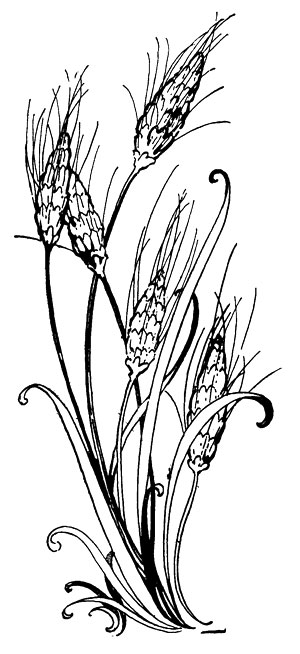
\includegraphics[width=0.45\textwidth]{image_011_2.jpg}
\end{wrapfigure}

\vspace{\onelineskip}

When she discovered

\vspace{\onelineskip}

that, she knew it ought

\vspace{\onelineskip}

to be planted. She was

\vspace{\onelineskip}

so busy hunting food for

\vspace{\onelineskip}

herself and her family

\vspace{\onelineskip}

that, naturally, she

\vspace{\onelineskip}

thought she ought not

\vspace{\onelineskip}

to take time to plant it.

\newpage
\begin{center}
	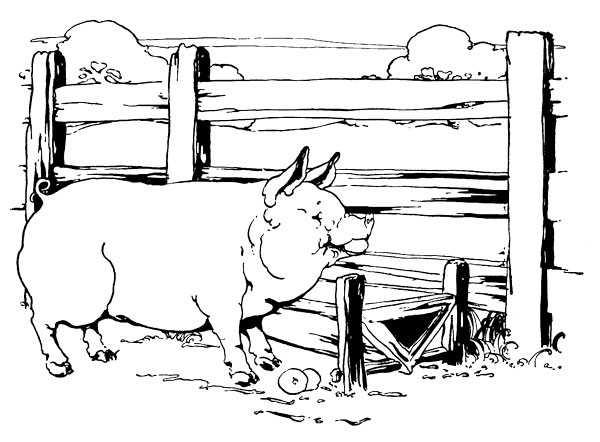
\includegraphics[width=\textwidth]{image_012_2.jpg}
\end{center}

\vspace{\onelineskip}

\begin{wrapfigure}[4]{l}{0.15\textwidth}
	\vspace{-\onelineskip}
	
\includegraphics[width=0.15\textwidth]{image_012_1.jpg}
\end{wrapfigure}

o she thought of the Pig—upon whom time must hang heavily and of the Cat
who had nothing to do, and of the great fat Rat with his idle hours, and
she called loudly:

\newpage
``Who will plant the Seed?''

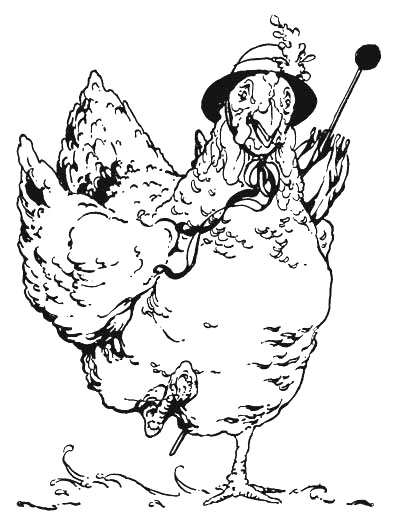
\includegraphics[width=0.8\textwidth]{image_004.jpg}

But the Pig said, ``Not I,''

and the Cat said, ``Not I,''

and the Rat said, ``Not I.''

\newpage
\begin{center}
	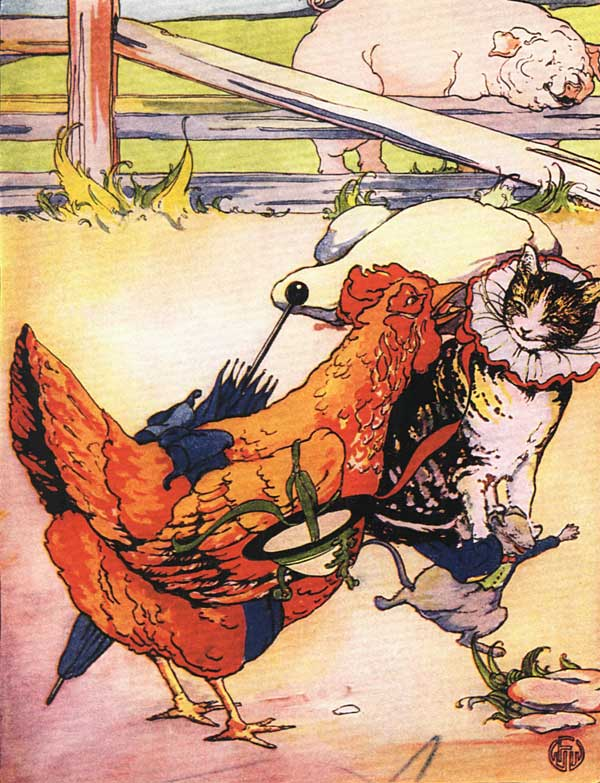
\includegraphics[width=\textwidth]{image_047_1.jpg}
\end{center}

\newpage
``Well, then,'' said the Little Red Hen, ``I will.''

\begin{center}
	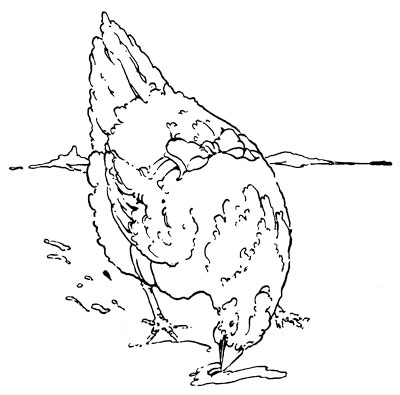
\includegraphics[width=\textwidth]{image_015.jpg}
\end{center}

And she did.

\newpage
\begin{center}
	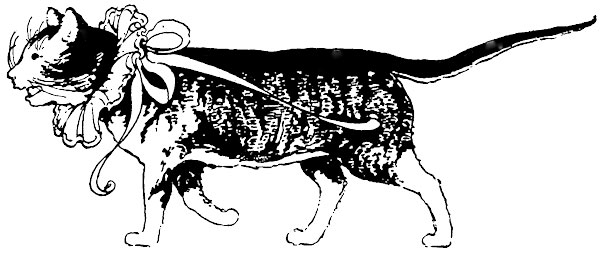
\includegraphics[width=0.7\textwidth]{image_016_1.jpg}
\end{center}

\begin{wrapfigure}[3]{l}{0.08\textwidth}
	\vspace{-1.25\onelineskip}
	
\includegraphics[width=0.1\textwidth]{image_016_2.jpg}
\end{wrapfigure}

hen she went on with her daily duties through the long summer days, scratching for worms and
feeding her chicks, while

\begin{wrapfigure}[5]{r}{0.5\textwidth}
	\vspace{-2\onelineskip}
	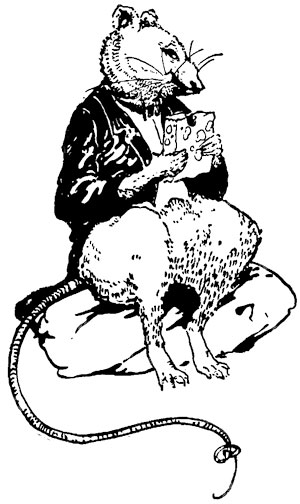
\includegraphics[width=0.5\textwidth]{image_016_3.jpg}
\end{wrapfigure}

\vspace{\onelineskip}

the Pig grew fat,

\vspace{\onelineskip}

and the Cat grew fat,

\vspace{\onelineskip}

and the Rat grew fat,

\vspace{\onelineskip}

and the Wheat

\vspace{\onelineskip}

grew tall and

\vspace{\onelineskip}

ready for

\vspace{\onelineskip}

harvest.

\newpage
\begin{wrapfigure}[4]{l}{0.15\textwidth}
	
\includegraphics[width=0.15\textwidth]{image_017_1.jpg}
\end{wrapfigure}

o one day the Little Red Hen chanced to notice how large the Wheat was and that the grain was
ripe, so she ran about calling briskly: “Who will cut the Wheat?”

\vspace{2\onelineskip}

The Pig said, “Not I,”

the Cat said, “Not I,”

and the Rat said, “Not I.”

\begin{wrapfigure}[4]{r}{0.7\textwidth}
	\vspace{-2\onelineskip}
	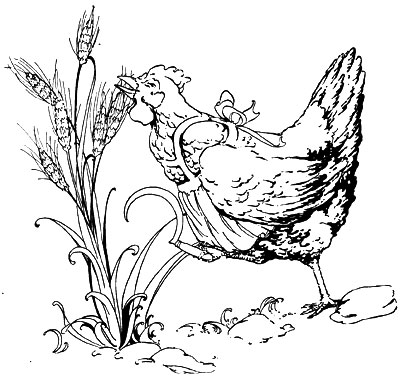
\includegraphics[width=0.7\textwidth]{image_017_2.jpg}
\end{wrapfigure}

\vspace{\onelineskip}

``Well,

\vspace{\onelineskip}

then,''

\vspace{\onelineskip}

said the

\vspace{\onelineskip}

Little

\vspace{\onelineskip}

Red Hen,

\vspace{\onelineskip}

``I will.''

\vspace{\onelineskip}

And she did.

\newpage
\begin{wrapfigure}[4]{l}{0.15\textwidth}
	
\includegraphics[width=0.15\textwidth]{image_017_1.jpg}
\end{wrapfigure}

he got the sickle from among the farmer's tools in the barn and proceeded to cut off all
of the big plant of Wheat.

\vspace{\onelineskip}

On the ground lay the nicely cut Wheat, ready to be gathered and threshed, but the newest
and yellowest and downiest of Mrs.

\begin{center}
	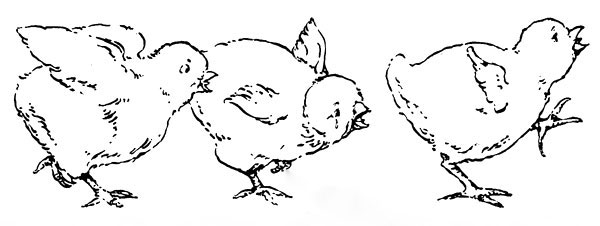
\includegraphics[width=\textwidth]{image_018_2.jpg}
\end{center}

Hen's chicks set up a “peep-peep-peeping” in their most vigorous fashion, proclaiming to the
world at large, but most particularly to their mother, that she was neglecting them.

\newpage
\begin{center}
	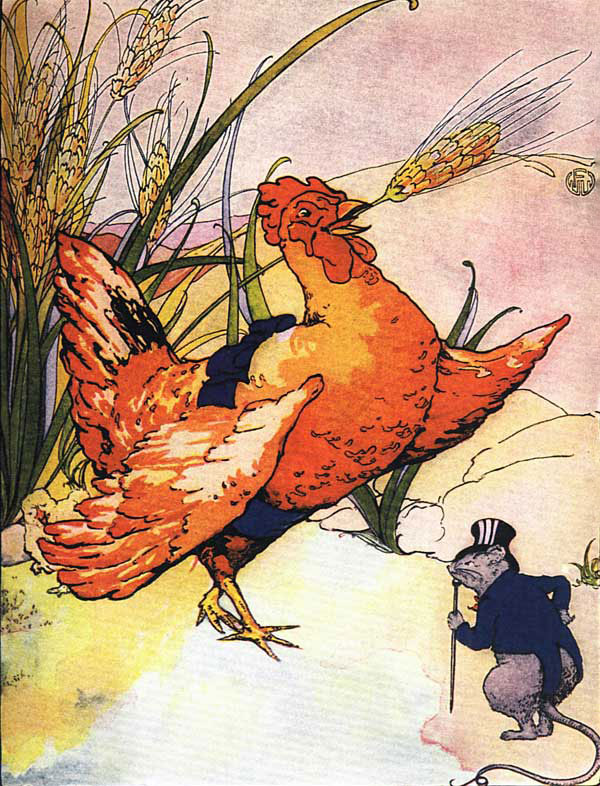
\includegraphics[width=\textwidth]{image_048_1.jpg}
\end{center}

\newpage
\begin{wrapfigure}[4]{l}{0.15\textwidth}
	
\includegraphics[width=0.15\textwidth]{image_020.jpg}
\end{wrapfigure}

oor Little Red Hen! She felt quite bewildered and hardly knew where to turn.

\vspace{\onelineskip}

Her attention was sorely divided between her duty to her children and her duty to the Wheat,
for which she felt responsible.

\vspace{\onelineskip}

So, again, in a very hopeful tone, she called out, ``Who will thresh the Wheat?''

\vspace{\onelineskip}

But the Pig, with a grunt, said, ``Not I,'' and the Cat, with a meow, said, ``Not I,'' and the Rat,
with a squeak, said, ``Not I.''

\vspace{\onelineskip}

So the Little Red Hen, looking, it must be admitted, rather discouraged, said, ``Well, I will,
then.''

\vspace{\onelineskip}

And she did.

\newpage
Of course, she had to feed her babies first, though, and when she had gotten them all to sleep for
their afternoon nap, she

\begin{center}
	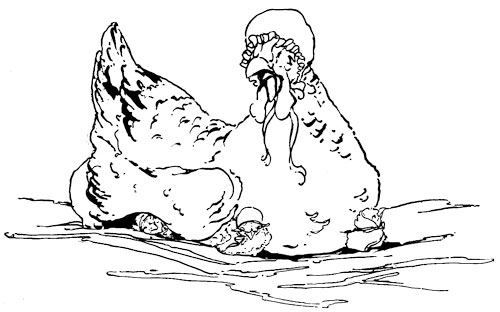
\includegraphics[width=\textwidth]{image_021.jpg}
\end{center}

went out and threshed the Wheat. Then she called out: ``Who will carry the Wheat to the mill to be
ground?''

\vspace{\onelineskip}

Turning their backs with snippy glee, that Pig said, ``Not I,''

\newpage
\begin{center}
	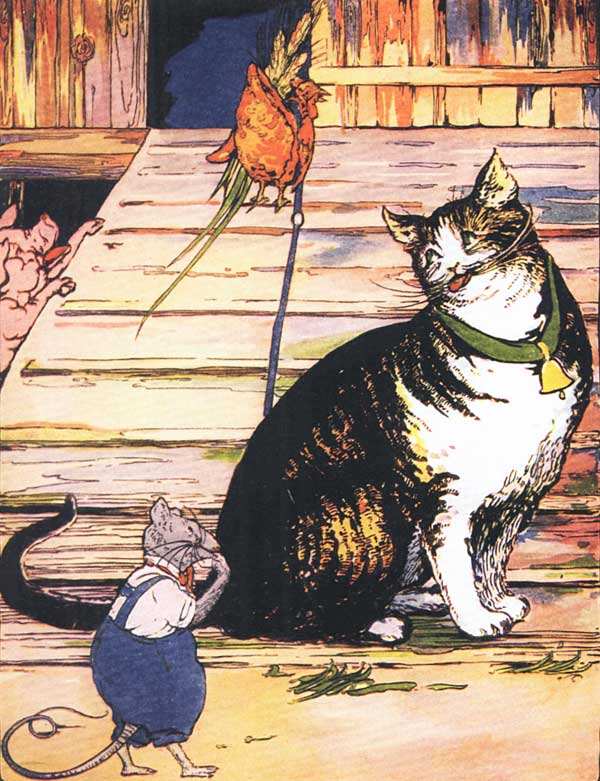
\includegraphics[width=\textwidth]{image_049_1.jpg}
\end{center}

\newpage
\begin{center}
	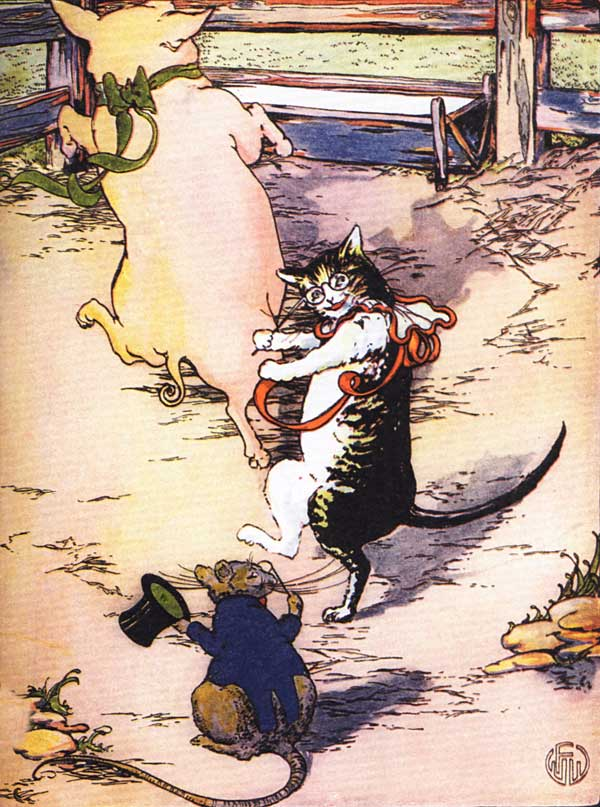
\includegraphics[width=\textwidth]{image_050_1.jpg}
\end{center}

\newpage
\begin{wrapfigure}[10]{l}{0.6\textwidth}
	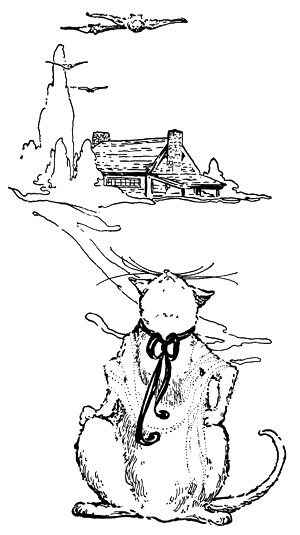
\includegraphics[width=0.6\textwidth]{image_024.jpg}
\end{wrapfigure}

and

\vspace{\onelineskip}

that

\vspace{\onelineskip}

Cat

\vspace{\onelineskip}

said,

\vspace{\onelineskip}

``Not I,''

\vspace{\onelineskip}

and

\vspace{\onelineskip}

that

\vspace{\onelineskip}

Rat

\vspace{\onelineskip}

said,

\vspace{\onelineskip}

``Not I.''

\newpage
\begin{wrapfigure}[4]{l}{0.15\textwidth}
	
\includegraphics[width=0.15\textwidth]{image_012_1.jpg}
\end{wrapfigure}
o the good Little Red Hen could do nothing but say, ``I will then.'' And she did.

\vspace{\onelineskip}

Carrying the sack of Wheat, she trudged off to the distant mill. There she ordered the Wheat
ground into beautiful white flour. When the miller brought her the

\vspace{\onelineskip}

\begin{wrapfigure}[10]{r}{0.7\textwidth}
	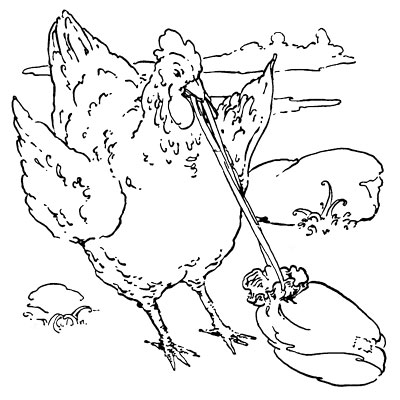
\includegraphics[width=0.7\textwidth]{image_025_2.jpg}
\end{wrapfigure}

flour she

\vspace{\onelineskip}

walked

\vspace{\onelineskip}

slowly

\vspace{\onelineskip}

back all

\vspace{\onelineskip}

the way

\vspace{\onelineskip}

to her own

\vspace{\onelineskip}

barnyard

\vspace{\onelineskip}

in her own

\vspace{\onelineskip}

picketty-pecketty

\vspace{\onelineskip}

fashion.

\newpage
\begin{center}
	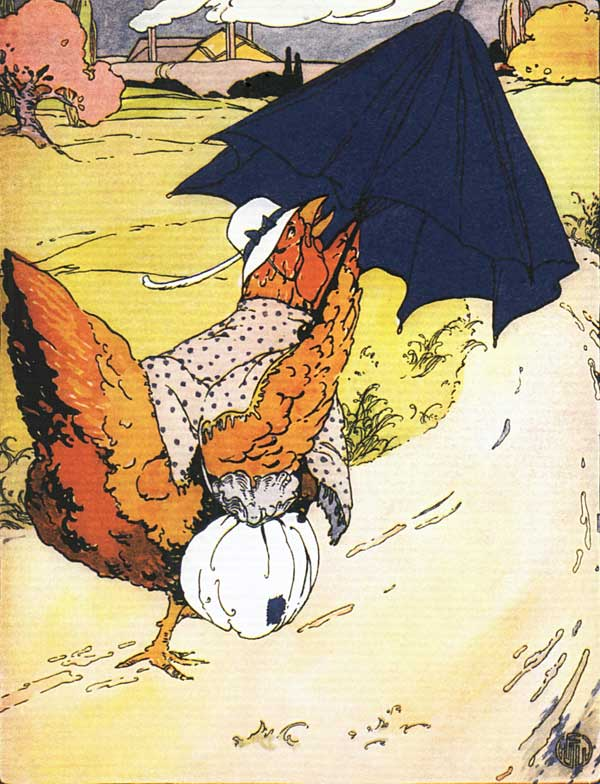
\includegraphics[width=\textwidth]{image_051_1.jpg}
\end{center}

\newpage
\begin{center}
	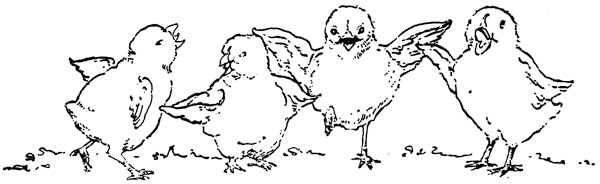
\includegraphics[width=\textwidth]{image_009_2.jpg}
\end{center}

\vspace{\onelineskip}
\begin{wrapfigure}[4]{l}{0.15\textwidth}
	\vspace{-2\onelineskip}
	
\includegraphics[width=0.15\textwidth]{image_017_1.jpg}
\end{wrapfigure}

he even managed, in spite of her load, to catch a nice juicy worm now and then and had one left
for the babies when she reached them. Those cunning little fluff-balls were \textit{so} glad to see
their mother. For the first time, they really appreciated her.

\vspace{\onelineskip}

\begin{center}
	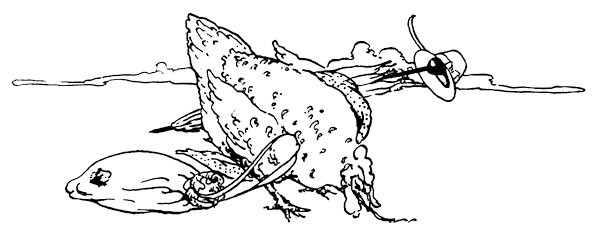
\includegraphics[width=\textwidth]{image_027_3.jpg}
\end{center}

\newpage
\begin{center}
	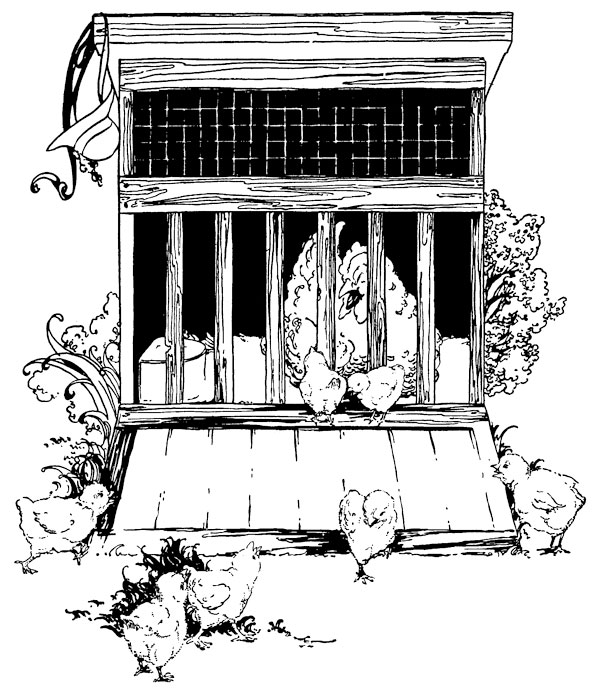
\includegraphics[width=0.7\textwidth]{image_028.jpg}
\end{center}

After this really strenuous day Mrs. Hen retired to her slumbers earlier than usual—indeed, before
the colors came into the sky to herald the setting of the sun, her usual bedtime hour.

\vspace{\onelineskip}

She would have liked to sleep late in the morning, but her chicks, joining in the morning chorus of
the hen yard, drove away all hopes of such a luxury.

\newpage
Even as she sleepily half opened one eye, the thought came to her that to-day that Wheat must,
somehow, be made into bread.

\begin{center}
	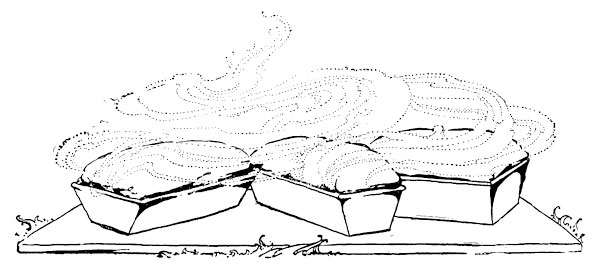
\includegraphics[width=\textwidth]{image_029.jpg}
\end{center}

\vspace{\onelineskip}

She was not in the habit of making bread, although, of course, anyone can make it if he or she
follows the recipe with care, and she knew perfectly well that she could do it if necessary.

\newpage
So after her children were fed and made sweet and fresh for the day, she hunted up the Pig, the
Cat and the Rat.

\vspace{\onelineskip}

Still confident that they would

\begin{wrapfigure}[6]{l}{0.7\textwidth}
	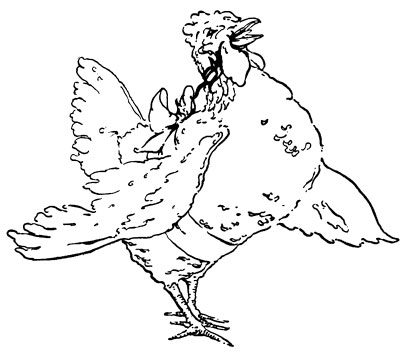
\includegraphics[width=0.7\textwidth]{image_030.jpg}
\end{wrapfigure}

surely help

\vspace{\onelineskip}

her some day

\vspace{\onelineskip}

she sang out,

\vspace{\onelineskip}

``Who will

\vspace{\onelineskip}

make the

\vspace{\onelineskip}

bread?''

\newpage
\begin{wrapfigure}[2]{l}{0.15\textwidth}
	
\includegraphics[width=0.15\textwidth]{image_005_1.jpg}
\end{wrapfigure}
as for the Little Red Hen! Once more her hopes were dashed! For the

\vspace{2\onelineskip}

\begin{wrapfigure}[9]{l}{0.7\textwidth}
	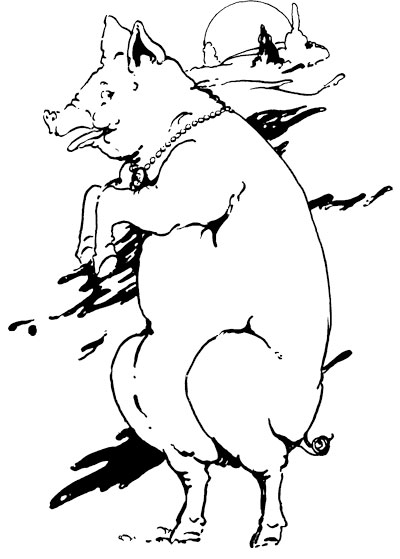
\includegraphics[width=0.7\textwidth]{image_031_2.jpg}
\end{wrapfigure}

Pig

\vspace{\onelineskip}

said,

\vspace{\onelineskip}

``Not

\vspace{\onelineskip}

I,''

\vspace{2\onelineskip}

the

\vspace{\onelineskip}

Cat

\vspace{\onelineskip}

said,

\vspace{\onelineskip}

``Not

\vspace{\onelineskip}

I,''

\newpage
\begin{wrapfigure}[6]{r}{0.6\textwidth}
	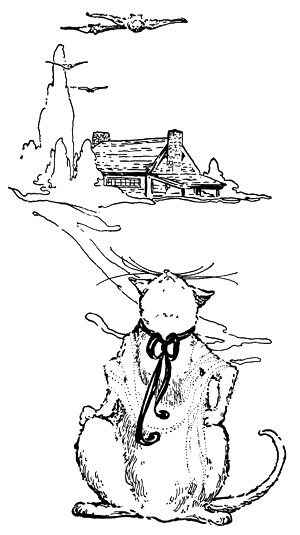
\includegraphics[width=0.6\textwidth]{image_024.jpg}
\end{wrapfigure}

and

\vspace{\onelineskip}

the

\vspace{\onelineskip}

Rat

\vspace{\onelineskip}

said,

\vspace{\onelineskip}

``Not

\vspace{\onelineskip}

I.''

\newpage
\begin{wrapfigure}[5]{l}{0.15\textwidth}
	
\includegraphics[width=0.15\textwidth]{image_012_1.jpg}
\end{wrapfigure}

o the Little Red Hen said once more, ``I will then,'' and she did.

\vspace{\onelineskip}

Feeling that she might have known all the time that she would have to do it all herself, she went and put on a fresh apron and spotless cook's cap. First of all she set the dough, as was proper. When it was time she brought out the moulding board and the baking tins, moulded the bread, divided it into loaves, and put them into the oven to bake. All the while the Cat sat lazily by, giggling and chuckling.

\newpage
\begin{center}
	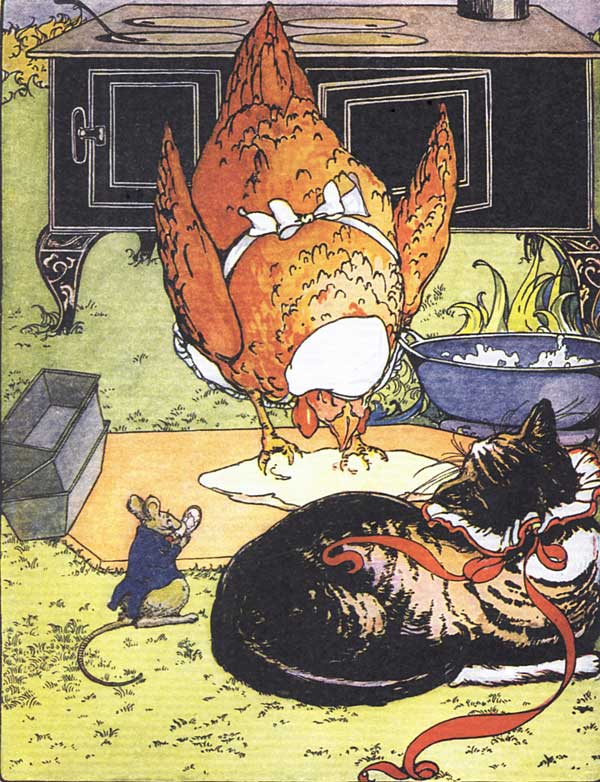
\includegraphics[width=\textwidth]{image_052_1.jpg}
\end{center}

\newpage
\begin{wrapfigure}[13]{l}{0.6\textwidth}
	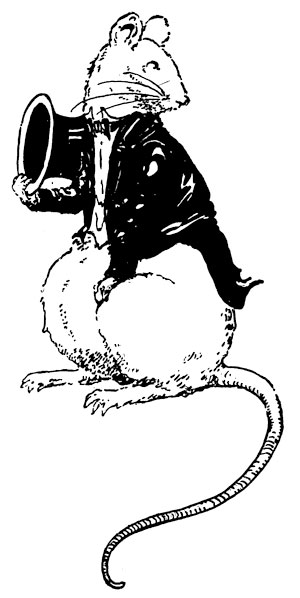
\includegraphics[width=0.6\textwidth]{image_008.jpg}
\end{wrapfigure}

And close at

\vspace{\onelineskip}

hand the

\vspace{\onelineskip}

vain Rat

\vspace{\onelineskip}

powdered

\vspace{\onelineskip}

his nose

\vspace{\onelineskip}

and admired

\vspace{\onelineskip}

himself

\vspace{\onelineskip}

in a mirror.

\vspace{\onelineskip}

In the distance

\vspace{\onelineskip}

could be

\vspace{\onelineskip}

heard the long-drawn

\vspace{\onelineskip}

snores of

\vspace{\onelineskip}

the dozing Pig.

\newpage
\begin{wrapfigure}[4]{l}{0.15\textwidth}
	
\includegraphics[width=0.15\textwidth]{image_005_1.jpg}
\end{wrapfigure}

t last the great moment arrived. A delicious odor was wafted upon the autumn breeze. Everywhere
the barnyard citizens sniffed the air with delight.

\begin{center}
	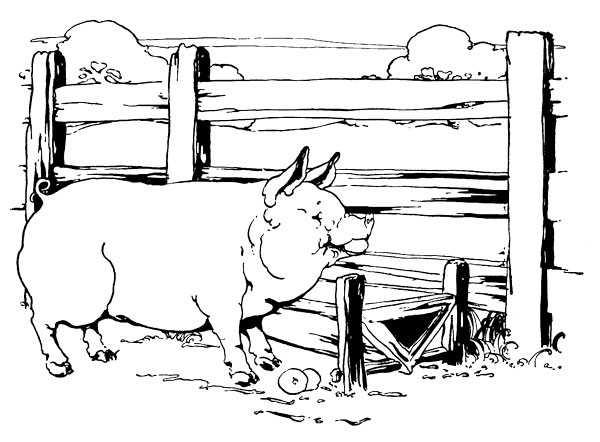
\includegraphics[width=\textwidth]{image_012_2.jpg}
\end{center}

\newpage
\begin{center}
	\includegraphics[width=0.8\textwidth]{image_037.jpg}
\end{center}
The Red Hen ambled in her picketty-pecketty way toward the source of all this excitement.

\newpage
\begin{wrapfigure}[3]{l}{0.15\textwidth}
	\includegraphics[width=0.15\textwidth]{image_005_1.jpg}
\end{wrapfigure}
lthough she appeared to be perfectly calm, in reality she could only with difficulty restrain an
impulse to dance and sing, for had she not

\vspace{2\onelineskip}
\begin{wrapfigure}[8]{l}{0.7\textwidth}
	\includegraphics[width=0.7\textwidth]{image_004.jpg}
\end{wrapfigure}

done

\vspace{\onelineskip}

all

\vspace{\onelineskip}

the

\vspace{\onelineskip}

work

\vspace{\onelineskip}

on

\vspace{\onelineskip}

this

\vspace{\onelineskip}

wonderful

\vspace{\onelineskip}

bread?

\newpage
\begin{wrapfigure}[5]{l}{0.15\textwidth}
	\includegraphics[width=0.15\textwidth]{image_017_1.jpg}
\end{wrapfigure}
mall wonder that she was the most excited person in the barnyard!

She did not know whether the bread would be fit to eat, but—joy of joys!—when the lovely brown
loaves came out of the oven,

\begin{center}
	\includegraphics[width=\textwidth]{image_029.jpg}
\end{center}

they were done to perfection.

\newpage
Then, probably because she had acquired the habit, the Red Hen called:

\vspace{\onelineskip}

\begin{wrapfigure}[5]{r}{0.7\textwidth}
	\includegraphics[width=0.7\textwidth]{image_030.jpg}
\end{wrapfigure}

``Who

\vspace{\onelineskip}

\indent\hspace{0.25cm} will

\vspace{\onelineskip}

\indent\hspace{0.5cm} eat

\vspace{\onelineskip}

\indent\hspace{0.75cm} the

\vspace{\onelineskip}

\indent\hspace{1cm} Bread?''

\newpage

All the animals in the barnyard were watching hungrily and smacking their lips in anticipation, and

\vspace{\onelineskip}

\indent\hspace{0.25cm} the Pig said, ``I will,''

\vspace{\onelineskip}

\indent\hspace{0.25cm} the Cat said, ``I will,''

\vspace{\onelineskip}

\indent\hspace{0.25cm} the Rat said, ``I will.''

\vspace{\onelineskip}

But the Little Red Hen said,

\begin{center}
	\includegraphics[width=\textwidth]{image_041.jpg}
\end{center}

\newpage
\begin{center}
	\includegraphics[width=\textwidth]{image_053_1.jpg}
\end{center}

\newpage

``No, you won't. I will.''

\vspace{3\onelineskip}

\begin{wrapfigure}[3]{l}{0.7\textwidth}
	\vspace{-2\onelineskip}
	\includegraphics[width=0.7\textwidth]{image_005_2.jpg}
\end{wrapfigure}

And

\vspace{4\onelineskip}

\indent\hspace{0.5cm} she

\vspace{4\onelineskip}

\indent\hspace{1cm} did.

\newpage
\begin{center}
	\includegraphics[width=\textwidth]{image_044.jpg}
\end{center}

\end{document}

